\section{Experiments}

\subsection{Benchmarks}

\subsubsection{Arcade Learning Environment}

The Arcade Learning Environment (ALE) has became a platform for evaluating artificial intelligence agents. Originally proposed by Bellemare et. al. \cite{Code.ALE}, the ALE makes available dozens of Atari 2600 games for an agent training and evaluation. The agent is expected to do well in as many games as possible without game-specific information, generally perceiving the world through a video stream. Atari 2600 games are excellent environments for evaluating AI agents for three main reasons: they are varied enough to provide multiple different tasks, requiring general competence, they are interesting and challenging for humans and they are free of experimenter’s bias, having been developed by an independent party.

In the context of the ALE, a discrete action is a number in range from 0 to 17 inclusive which encodes the composition of a joystick direction and an optional button press. The agent observes a reward signal, which is typically the change in the player’s score (the difference in score between the previous time step and the current time step), and an observation $o_t \in O$ of the environment. This observation can take form of a single 210 × 160 image and/or the current 1024-bit RAM state. Because a single image typically does not satisfy the Markov property the ALE is formalised as POMDP. Observations and the environment state are distinguished, with the RAM data being the real state of the emulator. A frame (as a unit of time) corresponds to 1/60th of a second, the time interval between two consecutive images rendered to the television screen. The ALE is deterministic, which means that given a particular emulator state $s$ and a action $a$ there is a unique next state $s'$, that is, $P^a_{ss'} = p(s' | s, a) = 1$.

Agents interact with the ALE in an episodic fashion. An episode begins by resetting the environment to its initial configuration, $s_0$, and ends at a given endpoint depending on a game. The primary measure of an agent’s performance is the score achieved during an episode, namely the undiscounted sum of rewards for that episode. While this performance measure is quite natural, it is important to realize that score is not necessarily an indicator of AI progress. In some games, agents can exploit the game's mechanics to maximize sum of rewards, but not complete the game's goal in human's understanding. \cite{Study.FaultyReward}

Preprocessing include frame skipping \cite{Study.FrameSkipping} which restricts the agent’s decision points by repeating a selected action for 4 consecutive frames. Frame skipping results in a simpler reinforcement learning problem and speeds up execution.
\editnote{TODO: Describe other preprocessing techniques used here.}

This work uses ALE through OpenAI Gym API \cite{Code.OpenAIGym}, specifically two games are used as benchmarks: Boxing and Freeway.

Boxing is a video game based on the sport of boxing. Boxing shows a top-down view of two boxers, one white and one black. When close enough, a boxer can hit his opponent with a punch. This causes his opponent to reel back slightly and the boxer scores a point, a reward of 1. In the other situation, when the boxer gets hit, he gets a negative reward of -1. There are no knockdowns or rounds. A match is completed either when one player lands 100 punches (a 'knockout') or two minutes have elapsed. In the case of a decision, the player with the most landed punches is the winner. Ties are possible. 
While the gameplay is simple, there are subtleties, such as getting an opponent on the 'ropes' and 'juggling' him back and forth between alternate punches. 

\begin{figure}[H]
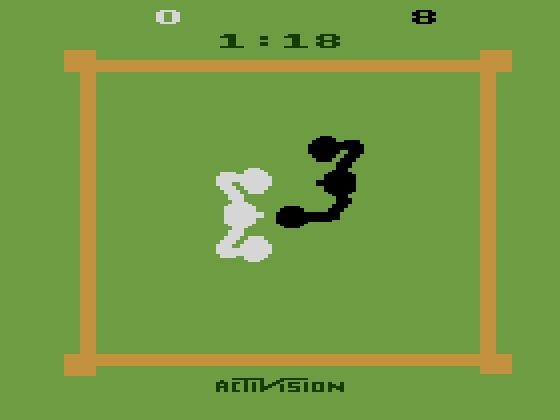
\includegraphics[width=0.5\textwidth,keepaspectratio]{figures/Boxing.jpg}
\caption[Sokoban]{Example of Boxing level}
\label{Fig.Boxing}
\end{figure}

In Freeway an agent controls a chicken who can be made to run across a ten lane highway filled with traffic in an effort to 'get to the other side.' Every time a chicken gets across a reward of 1 is earned by the agent. If hit by a car, then a chicken is forced back slightly. The goal is to score as much points as possible in the two minutes. The chicken is only allowed to move up or down. 
The major challenge in this environment are sparse rewards. The agent scores only when successfully crosses the highway, which isn't a trivial task.

\begin{figure}[H]
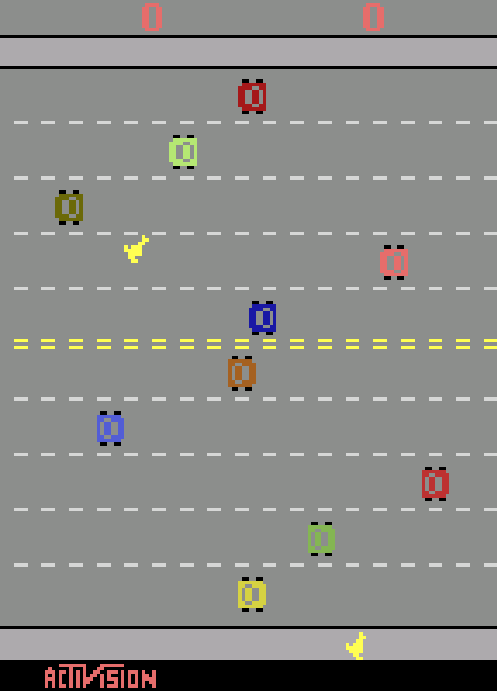
\includegraphics[width=0.5\textwidth,keepaspectratio]{figures/Freeway.png}
\caption[Sokoban]{Example of Freeway level}
\label{Fig.Boxing}
\end{figure}

\editnote{TODO: Add more games if needed.}

\subsubsection{Sokoban}

Sokoban is a classic planning problem. It is a challenging one-player puzzle game in which the goal is to navigate a grid world maze and push boxes onto target tiles. A Sokoban puzzle is considered solved when all boxes are positioned on top of target locations. The player can move in all 4 cardinal directions and only push boxes into an empty space (as opposed to pulling). For this reason many moves are irreversible and mistakes can render the puzzle unsolvable. A human player is thus forced to plan moves ahead of time. Artificial agents should similarly benefit from a learned model and simulation.

Despite its simple rule set, Sokoban is an incredibly complex game for which no general solver exists. It can be shown that Sokoban is NP-Hard and PSPACE-complete \cite{Benchmark.Sokoban}. Sokoban has an enormous state space that makes it inassailable to exhaustive search methods. An efficient automated solver for Sokoban must have strong heuristics, just as humans utilize their strong intuition, so that it is not overwhelmed by the number of possible game states.

The implementation of Sokoban\cite{Code.Sokoban} used for those experiments procedurally generates a new level each episode. This means an agent cannot memorize specific puzzles. Together with the planning aspect, this makes for a very challenging environment. While the underlying game logic operates in a 10 × 10 grid world, agents were trained directly on RGB sprite graphics. Fig.~\ref{Fig.Sokoban} shows an example of Sokoban level with 4 boxes and fig.~\ref{Fig.Sokoban_elements} explains the meaning of the visual icons.

\editnote{Note to the advisor: Do we need to go into deeper details about e.g. how rewards are obtained etc.? Or rather point to the repository for more information?}

\begin{figure}[H]
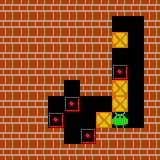
\includegraphics[]{figures/Sokoban.png}
\caption[Sokoban]{Example of Sokoban level (image size 160 × 160 pixels)}
\label{Fig.Sokoban}
\end{figure}

\subsection{Model learning}

First three experiments focus on training the world model in Sokoban environment. Because Sokoban is the deterministic environment, each experiment tested also the memory module without Mixture Density Network on top of a RNN. Instead a linear model was used to output the next latent state. \editnote{Note to the advisor: Should it be in the previous chapter (Planning with learned model a.k.a. project plan)?}

\subsubsection{Train the world model in the Sokoban environment}

In this experiment, the original world model was trained in the Sokoban environment. No modification to the original method described in the related work chapter was made, beyond addition of the deterministic variant of memory module.

The vision model successfully learned to encode high dimensional observations into low dimensional latent states. Fig.~\ref{Fig.Sokoban_vision} shows original observations (first and third columns) side by side with reconstructed observations from their encodings (second and fourth columns).

\begin{figure}[H]
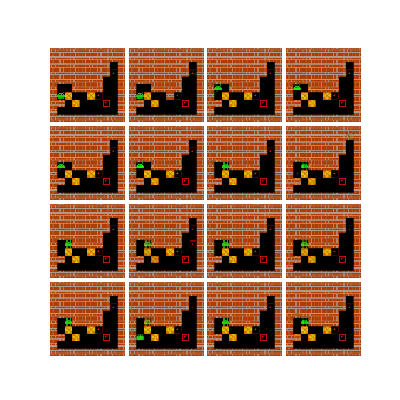
\includegraphics[width=1\textwidth,keepaspectratio]{figures/Sokoban_vision.png}
\caption[Qualitative result of the vision model training in Sokoban]{Qualitative result of the vision model training in Sokoban. First and third columns include original observations. Second and fourth columns include reconstructions. Each reconstruction was obtained by first encoding the original observation and then decoding, using VAE encoder and decoder respectively.}
\label{Fig.Sokoban_vision}
\end{figure}
\editnote{Make a better diagram.}

The stochastic and deterministic memory models were not able to learn Sokoban’s dynamics. Fig.~\ref{Fig.Sokoban_memory} shows that the stochastic model very often can not determine the agents position. The agent disappears and blocks change their types. The eighth row shows that pushing mechanics aren't modeled, the agent passes through boxes. The deterministic model don't do better.
The controller model failed to learn how to solve any level. We suspect that VAE is unable to generate usable abstract Sokoban representation and the shallow memory and controller models can not grasp complex dynamics of Sokoban using this poor representation.

\begin{figure}[H]
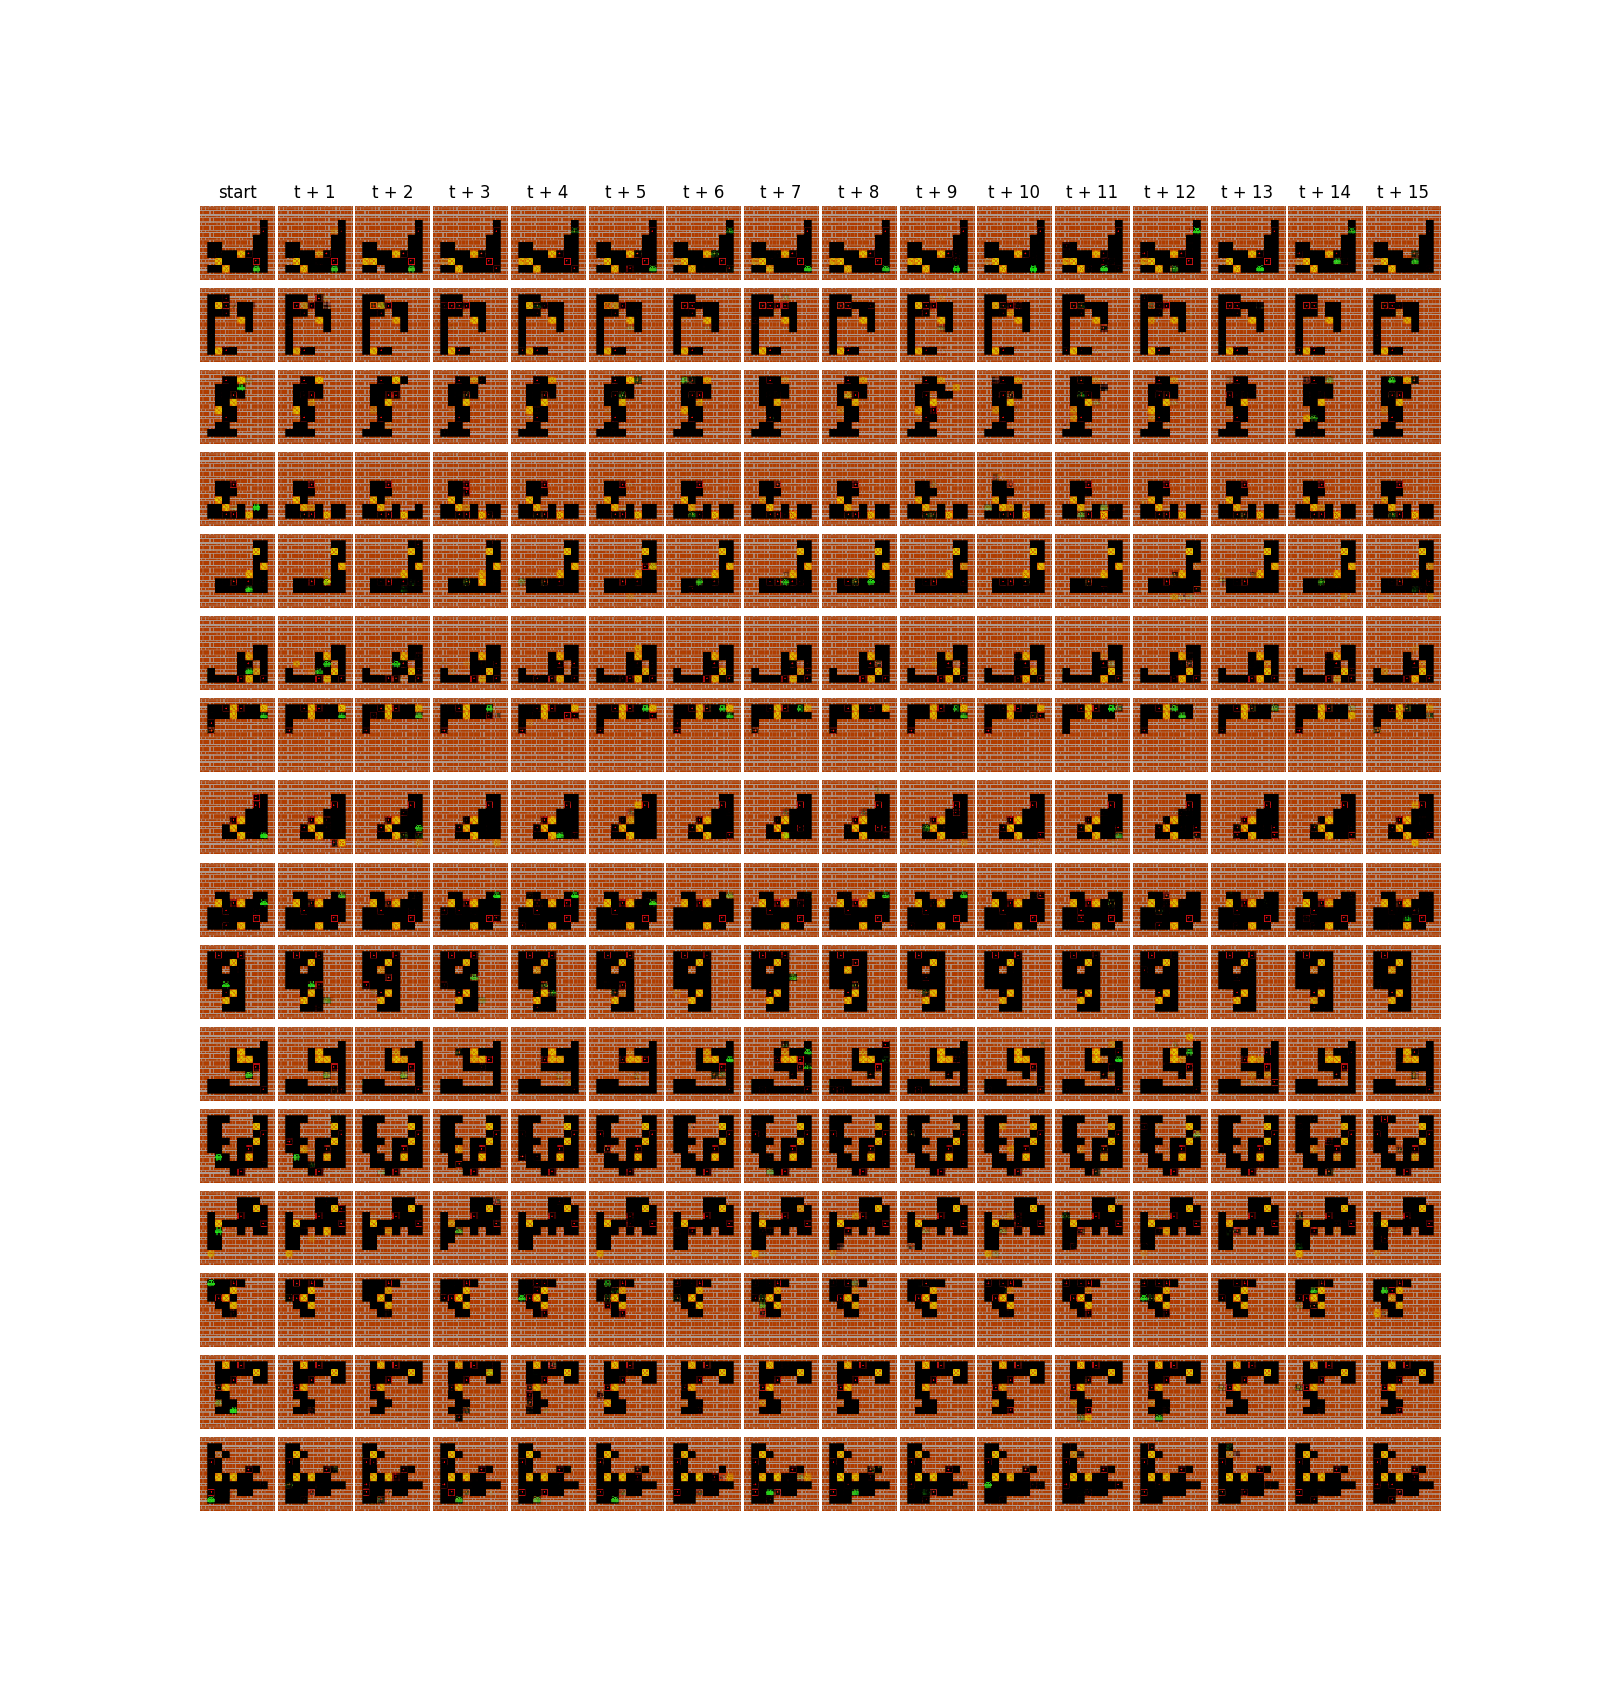
\includegraphics[width=1\textwidth,keepaspectratio]{figures/Sokoban_memory.png}
\caption[Qualitative result of the memory model training in Sokoban]{Qualitative result of the memory model training in Sokoban. Each row depicts the memory model rollout in one episode. The first column include original observations from the evaluation dataset from which the rollouts start. The RNN's hidden state was initialized on preceding transitions in each episode. Each subsequent reconstruction was obtained by first predicting the next latent state by the memory model and then decoding it using VAE decoder.}
\label{Fig.Sokoban_memory}
\end{figure}
\editnote{Make a better diagram.}
\editnote{Note to the advisor: Do we need to go into great detail about how it was generated? E.g. do we need to describe how the RNN was initialized or just point to the code?}

\subsubsection{Train the world model in Sokoban environment on 10x10 grid world states}

The latent state vector size is set to 64. This means that in theory this vector can accommodate full information about an observation. As noted before, Sokoban underlying game logic operates in a 10 × 10 grid world, where far edges of a level are always walls. This means that the level is described by 64 block types organized in an 8 x 8 grid. In this experiment, this domain knowledge is exploited and the agent uses those 64 block types as an input vector to the memory module, bypassing the vision model. It is worth noting, that the vision model should learn this representation as it is the optimal encoding when the objective is to compress a pixel image into a 64-dimensional vector and then reconstruct the original observation from it. However, despite use of the optimal encoding, the results have not been improved.

The proposed input format is optimal encoding if one wants to compress a pixel image and then reconstruct it. However, it is really poor representation of a current state of the environment if one wants to use linear combination of those features (block types in each position) to infer optimal next action and this is exactly what the controller model is tying to do. Modeling a value function could have more sense e.g. the value function could learn that a box on a target position yields higher value, but even it would have a hard time modeling more complex relations between entities in the environment. More useful for the controller would be e.g. representation that includes information about distance between the box and each target position. Nevertheless, this could be not enough too. The box on the target position would get discounted for not being on some other target positions. Hence, there is need for feature saying “the box X placed on the target position Y”. In the end, the linear combination of the proposed latent features can't model useful policy.

On the other hand, this representation includes, not well represented, but perfect information about an environment state. The memory model creates its own environment representation encoded in its hidden state and then uses this representation to predict the next latent state. This memory's hidden state is also utilized by the controller. Still, it doesn't seem to encode useful enough information for the two to do well on their tasks. One way to improve the hidden state representation is explored in the next experiment.

\subsubsection{Train the world model in Sokoban with auxiliary tasks}

Auxiliary tasks\cite{Algo.AuxiliaryTasks} have proved to help create more informative representation of an environment. In this experiment, reward and value prediction tasks are added to the memory model. In short, two additional linear models are added on top of the RNN to predict the next reward in the environment and model a value function. In theory, it should help form a more informative hidden state of the memory model. Consequently, it should help learn Sokoban’s dynamics, but also generate representation on a higher level of abstraction that could prove useful for the controller. Moreover, a reward prediction will be needed in further work on planning with learned model.

For all that, the memory model have not been able to learn to predict the rewards and values. Also, there was no improvement in memory's and controller’s performance. It is suspected, that the main cause of this failure are sparse rewards in the training dataset. A random agent used to generate the dataset does not receive many positive rewards. Effectively, most of the episodes do not have any positive reward. Hence, the memory model soon overfit on more or less constant reward and value. 
This yields insight that the data generation procedure does not cover state-space well. Iterative approach to gathering data, from a better and better agent, could solve this problem.

It is not without significance that Sokoban has enormous state-space. Each episode is much different from the others - it is nearly impossible for an agent to see a similar state in a different episode. Hence, Sokoban requires strong generalization capability from the memory module. Simple RNN can lack capacity to create good representation and in turn achieve good prediction performance. For instance I2A\cite{Algo.I2A} uses deep neural network architecture to handle Sokoban complexity. A more flexible memory model with larger capacity could manage this complexity and need for generalization. We explore those two insights in the next experiment with larger model and iterative training procedure.
